\section{UAbstract\-Client Class Reference}
\label{classUAbstractClient}\index{UAbstractClient@{UAbstractClient}}
Interface for an URBI wrapper object.  


{\tt \#include $<$uabstractclient.h$>$}

Inheritance diagram for UAbstract\-Client::\begin{figure}[H]
\begin{center}
\leavevmode
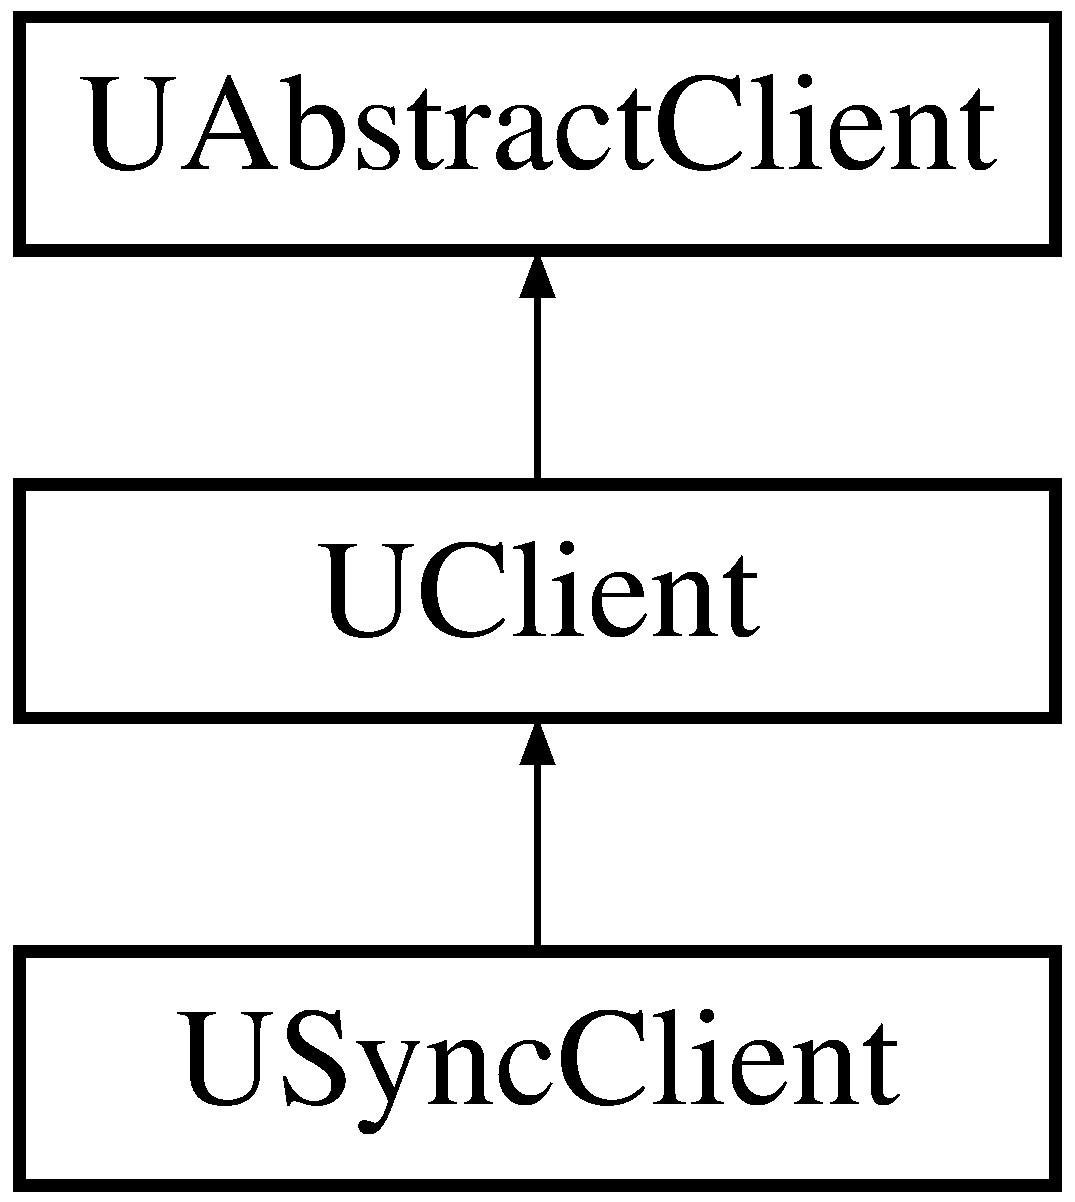
\includegraphics[height=3cm]{classUAbstractClient}
\end{center}
\end{figure}
\subsection*{Public Member Functions}
\begin{CompactItemize}
\item 
{\bf UAbstract\-Client} (const char $\ast$\_\-host, int \_\-port={\bf URBI\_\-PORT}, int \_\-buflen={\bf URBI\_\-BUFLEN})
\begin{CompactList}\small\item\em Create a new instance and connect to the Urbi server. \item\end{CompactList}\item 
int {\bf error} ()\label{classUAbstractClient_a2}

\begin{CompactList}\small\item\em Return current error status, or zero if no error occurred. \item\end{CompactList}\item 
int {\bf send} ()\label{classUAbstractClient_a3}

\begin{CompactList}\small\item\em Function for backward compatibility. Will be removed in future versions. \item\end{CompactList}\item 
int {\bf send} (const char $\ast$format,...)
\begin{CompactList}\small\item\em Send an Urbi command. The syntax is similar to the {\bf printf()}{\rm (p.\,\pageref{classUAbstractClient_a31})} function. \item\end{CompactList}\item 
int {\bf send\-Bin} (const void $\ast$, int len)\label{classUAbstractClient_a5}

\begin{CompactList}\small\item\em Send binary data. \item\end{CompactList}\item 
int {\bf send\-Bin} (const void $\ast$, int len, const char $\ast$header,...)\label{classUAbstractClient_a6}

\begin{CompactList}\small\item\em Send an Urbi header followed by binary data. \item\end{CompactList}\item 
int {\bf start\-Pack} ()
\begin{CompactList}\small\item\em Lock the send buffer (for backward compatibility, will be removed in future versions). \item\end{CompactList}\item 
int {\bf end\-Pack} ()\label{classUAbstractClient_a8}

\begin{CompactList}\small\item\em Unlock the send buffer (for backward compatibility, will be removed in future versions). \item\end{CompactList}\item 
int {\bf pack} (const char $\ast$,...)
\begin{CompactList}\small\item\em Append Urbi commands to the send buffer (for backward compatibility, will be removed in future versions). \item\end{CompactList}\item 
int {\bf vpack} (const char $\ast$, va\_\-list args)\label{classUAbstractClient_a10}

\begin{CompactList}\small\item\em va\_\-list version of pack. \item\end{CompactList}\item 
int {\bf send\-File} (const char $\ast$filename)\label{classUAbstractClient_a11}

\begin{CompactList}\small\item\em Send urbi commands contained in a file. \item\end{CompactList}\item 
UCallback\-ID {\bf send\-Command} ({\bf UCallback}, const char $\ast$,...)\label{classUAbstractClient_a12}

\begin{CompactList}\small\item\em Send a command, prefixing it with a tag, and associate the given callback with this tag. $\ast$/. \item\end{CompactList}\item 
UCallback\-ID {\bf send\-Command} (UCustom\-Callback, void $\ast$, const char $\ast$,...)\label{classUAbstractClient_a13}

\begin{CompactList}\small\item\em Send a command, prefixing it with a tag, and associate the given callback with this tag. $\ast$/. \item\end{CompactList}\item 
int {\bf send\-Sound} (const char $\ast$device, const {\bf USound} \&sound, const char $\ast$tag=0)
\begin{CompactList}\small\item\em Send sound data to the robot for immediate playback. \item\end{CompactList}\item 
int {\bf put\-File} (const char $\ast$local\-Name, const char $\ast$remote\-Name=0)\label{classUAbstractClient_a15}

\begin{CompactList}\small\item\em Put a file on the robot's mass storage device. \item\end{CompactList}\item 
int {\bf put\-File} (const void $\ast$buffer, int length, const char $\ast$remote\-Name)\label{classUAbstractClient_a16}

\begin{CompactList}\small\item\em Save a buffer to a file on the robot. \item\end{CompactList}\item 
UCallback\-ID {\bf set\-Callback} (UCallback\-Wrapper \&callback, const char $\ast$tag)\label{classUAbstractClient_a17}

\begin{CompactList}\small\item\em Associate a callback function with a tag. new style. \item\end{CompactList}\item 
UCallback\-ID {\bf set\-Error\-Callback} (UCallback\-Wrapper \&callback)\label{classUAbstractClient_a18}

\begin{CompactList}\small\item\em Associate a callbaxk function with all error messages. \item\end{CompactList}\item 
UCallback\-ID {\bf set\-Wildcard\-Callback} (UCallback\-Wrapper \&callback)\label{classUAbstractClient_a19}

\begin{CompactList}\small\item\em Associate a callback with all messages. \item\end{CompactList}\item 
UCallback\-ID {\bf set\-Callback} ({\bf UCallback}, const char $\ast$tag)\label{classUAbstractClient_a20}

\begin{CompactList}\small\item\em OLD-style callbacks. \item\end{CompactList}\item 
UCallback\-ID {\bf set\-Callback} (UCustom\-Callback, void $\ast$callback\-Data, const char $\ast$tag)\label{classUAbstractClient_a21}

\begin{CompactList}\small\item\em Associate a callback function with a tag, specifiing a callback custom value that will be passed back to the callback function. \item\end{CompactList}\item 
template$<$class C$>$ UCallback\-ID {\bf set\-Callback} (C \&ref, {\bf UCallback\-Action}(C::$\ast$)(const {\bf UMessage} \&), const char $\ast$tag)\label{classUAbstractClient_a22}

\begin{CompactList}\small\item\em Callback to class member functions(old-style). \item\end{CompactList}\item 
template$<$class C, class P1$>$ UCallback\-ID {\bf set\-Callback} (C \&ref, {\bf UCallback\-Action}(C::$\ast$)(P1, const {\bf UMessage} \&), P1, const char $\ast$tag)\label{classUAbstractClient_a23}

\item 
template$<$class C, class P1, class P2$>$ UCallback\-ID {\bf set\-Callback} (C \&ref, {\bf UCallback\-Action}(C::$\ast$)(P1, P2, const {\bf UMessage} \&), P1, P2, const char $\ast$tag)\label{classUAbstractClient_a24}

\item 
template$<$class C, class P1, class P2, class P3$>$ UCallback\-ID {\bf set\-Callback} (C \&ref, {\bf UCallback\-Action}(C::$\ast$)(P1, P2, P3, const {\bf UMessage} \&), P1, P2, P3, const char $\ast$tag)\label{classUAbstractClient_a25}

\item 
template$<$class C, class P1, class P2, class P3, class P4$>$ UCallback\-ID {\bf set\-Callback} (C \&ref, {\bf UCallback\-Action}(C::$\ast$)(P1, P2, P3, P4, const {\bf UMessage} \&), P1, P2, P3, P4, const char $\ast$tag)\label{classUAbstractClient_a26}

\item 
int {\bf get\-Associated\-Tag} (UCallback\-ID id, char $\ast$tag)
\begin{CompactList}\small\item\em Get the tag associated with a registered callback. \item\end{CompactList}\item 
int {\bf delete\-Callback} (UCallback\-ID call\-Back\-ID)
\begin{CompactList}\small\item\em Delete a callback. \item\end{CompactList}\item 
void {\bf make\-Unique\-Tag} (char $\ast$tag)\label{classUAbstractClient_a29}

\begin{CompactList}\small\item\em Fill tag with a unique tag for this client. \item\end{CompactList}\item 
void {\bf notify\-Callbacks} (const {\bf UMessage} \&msg)
\begin{CompactList}\small\item\em Simulate an Urbi message. \item\end{CompactList}\item 
virtual void {\bf printf} (const char $\ast$format,...)=0\label{classUAbstractClient_a31}

\begin{CompactList}\small\item\em Notify of an error. \item\end{CompactList}\item 
virtual unsigned int {\bf get\-Current\-Time} ()=0\label{classUAbstractClient_a32}

\begin{CompactList}\small\item\em Get time in milliseconds since an unspecified but constant reference time. \item\end{CompactList}\item 
virtual void {\bf lock\-Send} ()=0\label{classUAbstractClient_a33}

\begin{CompactList}\small\item\em Lock the send buffer for exclusive use by the current thread. \item\end{CompactList}\item 
virtual void {\bf unlock\-Send} ()=0\label{classUAbstractClient_a34}

\begin{CompactList}\small\item\em Unlock the send buffer. \item\end{CompactList}\item 
const char $\ast$ {\bf get\-Server\-Name} ()\label{classUAbstractClient_a35}

\begin{CompactList}\small\item\em Return the server name or IP address. \item\end{CompactList}\item 
template$<$class C, class P1$>$ UCallback\-ID {\bf set\-Callback} (C \&ref, {\bf UCallback\-Action}(C::$\ast$func)(P1, const {\bf UMessage} \&), P1 p1, const char $\ast$tag)\label{classUAbstractClient_a36}

\item 
template$<$class C, class P1, class P2$>$ UCallback\-ID {\bf set\-Callback} (C \&ref, {\bf UCallback\-Action}(C::$\ast$func)(P1, P2, const {\bf UMessage} \&), P1 p1, P2 p2, const char $\ast$tag)\label{classUAbstractClient_a37}

\item 
template$<$class C, class P1, class P2, class P3$>$ UCallback\-ID {\bf set\-Callback} (C \&ref, {\bf UCallback\-Action}(C::$\ast$func)(P1, P2, P3, const {\bf UMessage} \&), P1 p1, P2 p2, P3 p3, const char $\ast$tag)\label{classUAbstractClient_a38}

\end{CompactItemize}
\subsection*{Protected Member Functions}
\begin{CompactItemize}
\item 
void {\bf process\-Recv\-Buffer} ()
\begin{CompactList}\small\item\em Called each time new data is available in recv\-Buffer. \item\end{CompactList}\item 
virtual int {\bf effective\-Send} (const void $\ast$buffer, int size)=0\label{classUAbstractClient_b1}

\begin{CompactList}\small\item\em Queue data for sending, returns zero on success, nonzero on failure. \item\end{CompactList}\item 
virtual bool {\bf can\-Send} (int size)=0\label{classUAbstractClient_b2}

\begin{CompactList}\small\item\em Check if successive {\bf effective\-Send()}{\rm (p.\,\pageref{classUAbstractClient_b1})} of cumulated size 'size' will succeed. \item\end{CompactList}\item 
virtual void {\bf lock\-List} ()=0\label{classUAbstractClient_b3}

\begin{CompactList}\small\item\em Lock receive and send portions of the code. \item\end{CompactList}\item 
virtual void {\bf unlock\-List} ()=0\label{classUAbstractClient_b4}

\begin{CompactList}\small\item\em Unlock receive and send portions of the code. \item\end{CompactList}\item 
UCallback\-ID {\bf add\-Callback} (const char $\ast$tag, UCallback\-Wrapper \&w)\label{classUAbstractClient_b5}

\begin{CompactList}\small\item\em Add a callback to the list. \item\end{CompactList}\end{CompactItemize}
\subsection*{Protected Attributes}
\begin{CompactItemize}
\item 
char $\ast$ {\bf host}\label{classUAbstractClient_p0}

\begin{CompactList}\small\item\em Host name. \item\end{CompactList}\item 
int {\bf port}\label{classUAbstractClient_p1}

\begin{CompactList}\small\item\em URBI Port. \item\end{CompactList}\item 
int {\bf buflen}\label{classUAbstractClient_p2}

\begin{CompactList}\small\item\em URBI Buffer length. \item\end{CompactList}\item 
int {\bf rc}\label{classUAbstractClient_p3}

\begin{CompactList}\small\item\em System calls return value storage. \item\end{CompactList}\item 
char $\ast$ {\bf recv\-Buffer}\label{classUAbstractClient_p4}

\begin{CompactList}\small\item\em Reception buffer. \item\end{CompactList}\item 
int {\bf recv\-Buffer\-Position}\label{classUAbstractClient_p5}

\begin{CompactList}\small\item\em Current position in reception buffer. \item\end{CompactList}\end{CompactItemize}
\subsection*{Friends}
\begin{CompactItemize}
\item 
class {\bf UClient\-Streambuf}\label{classUAbstractClient_n0}

\end{CompactItemize}


\subsection{Detailed Description}
Interface for an URBI wrapper object. 

Implementations of this interface are wrappers around the URBI protocol. It handles URBI messages parsing, callback registration and various formatting functions. Implementations of this interface should:\begin{itemize}
\item Redefine error\-Notify() as a function able to notify the user of eventual errors.\item Redfine the four mutual exclusion functions.\item Redefine {\bf effective\-Send()}{\rm (p.\,\pageref{classUAbstractClient_b1})}.\item Fill recv\-Buffer, update recv\-Buffer\-Position and call {\bf process\-Recv\-Buffer()}{\rm (p.\,\pageref{classUAbstractClient_b0})} when new data is available.\item Provide an {\bf execute()}{\rm (p.\,\pageref{namespaceurbi_a5})} function in the namespace urbi, that never returns, and that will be called after initialization.\end{itemize}


See the liburbi-cpp documentation for more informations on how to use this class. 



Definition at line 229 of file uabstractclient.h.

\subsection{Constructor \& Destructor Documentation}
\index{UAbstractClient@{UAbstract\-Client}!UAbstractClient@{UAbstractClient}}
\index{UAbstractClient@{UAbstractClient}!UAbstractClient@{UAbstract\-Client}}
\subsubsection{\setlength{\rightskip}{0pt plus 5cm}UAbstract\-Client::UAbstract\-Client (const char $\ast$ {\em \_\-host}, int {\em \_\-port} = {\tt {\bf URBI\_\-PORT}}, int {\em \_\-buflen} = {\tt {\bf URBI\_\-BUFLEN}})}\label{classUAbstractClient_a0}


Create a new instance and connect to the Urbi server. 

Initializes send\-Buffer and recv\-Buffer, and copy \_\-host and \_\-port. \begin{Desc}
\item[Parameters:]
\begin{description}
\item[{\em \_\-host}]IP address or name of the robot to connect to. \item[{\em \_\-port}]TCP port to connect to. \item[{\em \_\-buflen}]size of send and receive buffers. Implementations should establish the connection in their constructor. \end{description}
\end{Desc}


Definition at line 166 of file uabstractclient.cpp.

References buflen, host, port, rc, and recv\-Buffer.

\subsection{Member Function Documentation}
\index{UAbstractClient@{UAbstract\-Client}!deleteCallback@{deleteCallback}}
\index{deleteCallback@{deleteCallback}!UAbstractClient@{UAbstract\-Client}}
\subsubsection{\setlength{\rightskip}{0pt plus 5cm}int UAbstract\-Client::delete\-Callback (UCallback\-ID {\em callback\-ID})}\label{classUAbstractClient_a28}


Delete a callback. 

Returns 0 if no callback with this id was found, 1 otherwise. 

Definition at line 544 of file uabstractclient.cpp.

References lock\-List(), and unlock\-List().

Referenced by send\-Command(), and send\-Sound().\index{UAbstractClient@{UAbstract\-Client}!getAssociatedTag@{getAssociatedTag}}
\index{getAssociatedTag@{getAssociatedTag}!UAbstractClient@{UAbstract\-Client}}
\subsubsection{\setlength{\rightskip}{0pt plus 5cm}int UAbstract\-Client::get\-Associated\-Tag (UCallback\-ID {\em id}, char $\ast$ {\em tag})}\label{classUAbstractClient_a27}


Get the tag associated with a registered callback. 

Returns 1 and fills tag on success, 0 on failure 

Definition at line 528 of file uabstractclient.cpp.

References lock\-List(), and unlock\-List().\index{UAbstractClient@{UAbstract\-Client}!notifyCallbacks@{notifyCallbacks}}
\index{notifyCallbacks@{notifyCallbacks}!UAbstractClient@{UAbstract\-Client}}
\subsubsection{\setlength{\rightskip}{0pt plus 5cm}void UAbstract\-Client::notify\-Callbacks (const {\bf UMessage} \& {\em msg})}\label{classUAbstractClient_a30}


Simulate an Urbi message. 

Pass the given {\bf UMessage}{\rm (p.\,\pageref{classUMessage})} to all registered callbacks with the corresponding tag, as if it were comming from the URBI server. 

Definition at line 140 of file uabstractclient.cpp.

References lock\-List(), UMessage::tag, UMessage::type, UCallback\-Action, and unlock\-List().

Referenced by process\-Recv\-Buffer().\index{UAbstractClient@{UAbstract\-Client}!pack@{pack}}
\index{pack@{pack}!UAbstractClient@{UAbstract\-Client}}
\subsubsection{\setlength{\rightskip}{0pt plus 5cm}int UAbstract\-Client::pack (const char $\ast$ {\em command},  {\em ...})}\label{classUAbstractClient_a9}


Append Urbi commands to the send buffer (for backward compatibility, will be removed in future versions). 

This function must only be called between a {\bf start\-Pack()}{\rm (p.\,\pageref{classUAbstractClient_a7})} and the corresponding {\bf end\-Pack()}{\rm (p.\,\pageref{classUAbstractClient_a8})}. Data is queued in the send buffer, and sent when {\bf end\-Pack()}{\rm (p.\,\pageref{classUAbstractClient_a8})} is called. 

Definition at line 257 of file uabstractclient.cpp.

References rc, and vpack().\index{UAbstractClient@{UAbstract\-Client}!processRecvBuffer@{processRecvBuffer}}
\index{processRecvBuffer@{processRecvBuffer}!UAbstractClient@{UAbstract\-Client}}
\subsubsection{\setlength{\rightskip}{0pt plus 5cm}void UAbstract\-Client::process\-Recv\-Buffer ()\hspace{0.3cm}{\tt  [protected]}}\label{classUAbstractClient_b0}


Called each time new data is available in recv\-Buffer. 

As long as this function has not returned, neither recv\-Buffer nor recv\-Buffer\-Pos may be modified. 

Definition at line 654 of file uabstractclient.cpp.

References lock\-List(), notify\-Callbacks(), printf(), recv\-Buffer, recv\-Buffer\-Position, and unlock\-List().

Referenced by UClient::listen\-Thread().\index{UAbstractClient@{UAbstract\-Client}!send@{send}}
\index{send@{send}!UAbstractClient@{UAbstract\-Client}}
\subsubsection{\setlength{\rightskip}{0pt plus 5cm}int UAbstract\-Client::send (const char $\ast$ {\em command},  {\em ...})}\label{classUAbstractClient_a4}


Send an Urbi command. The syntax is similar to the {\bf printf()}{\rm (p.\,\pageref{classUAbstractClient_a31})} function. 

Multiple commands can be sent in one call. 

Definition at line 234 of file uabstractclient.cpp.

References effective\-Send(), lock\-Send(), rc, unlock\-Send(), and vpack().\index{UAbstractClient@{UAbstract\-Client}!sendSound@{sendSound}}
\index{sendSound@{sendSound}!UAbstractClient@{UAbstract\-Client}}
\subsubsection{\setlength{\rightskip}{0pt plus 5cm}int UAbstract\-Client::send\-Sound (const char $\ast$ {\em device}, const {\bf USound} \& {\em sound}, const char $\ast$ {\em tag} = {\tt 0})}\label{classUAbstractClient_a14}


Send sound data to the robot for immediate playback. 

If tag is set, an URBI system \char`\"{}stop\char`\"{} message with this tag will be generated when the sound has been played. The sound data is copied in case of asynchronous send, and may be safely deleted as soon as this function returns. 

Definition at line 469 of file uabstractclient.cpp.

References USound::channels, USound::data, delete\-Callback(), make\-Unique\-Tag(), USound::rate, USound::sample\-Format, USound::sample\-Size, send\-Bin(), set\-Callback(), USound::size, and USound::sound\-Format.\index{UAbstractClient@{UAbstract\-Client}!startPack@{startPack}}
\index{startPack@{startPack}!UAbstractClient@{UAbstract\-Client}}
\subsubsection{\setlength{\rightskip}{0pt plus 5cm}int UAbstract\-Client::start\-Pack ()}\label{classUAbstractClient_a7}


Lock the send buffer (for backward compatibility, will be removed in future versions). 

In threaded environnments, this function locks the send buffer so that only the calling thread can call the send functions. Otherwise do nothing. 

Definition at line 215 of file uabstractclient.cpp.

References lock\-Send().

The documentation for this class was generated from the following files:\begin{CompactItemize}
\item 
{\bf uabstractclient.h}\item 
{\bf uabstractclient.cpp}\end{CompactItemize}
